\documentclass{beamer}
\usepackage{beamerthemesplit} % new

\usepackage[utf8]{inputenc}

\begin{document}
\title{Perdidos en la ignorancia}
\author{ES\_2019\_G43-2-02}
\date{\today}

\frame{\titlepage}

{\tiny \frame{\frametitle{Table of contents}\tableofcontents}}


\section{Membres del equip}
\frame{\frametitle{Team}
  \begin{itemize}
    \item Aleksandra Jovanovic
    \item Daniel Montesinos Santos
    \item Adrián Moreno Gimeno
    \item Núria Navarro Juliana
    \item Desirée Pasión Rodriguez Sanchez
  \end{itemize}
}


\section{Jira}
%\subsection{Product Backlog/Tasques}
%\frame{\frametitle{Product Backlog}
%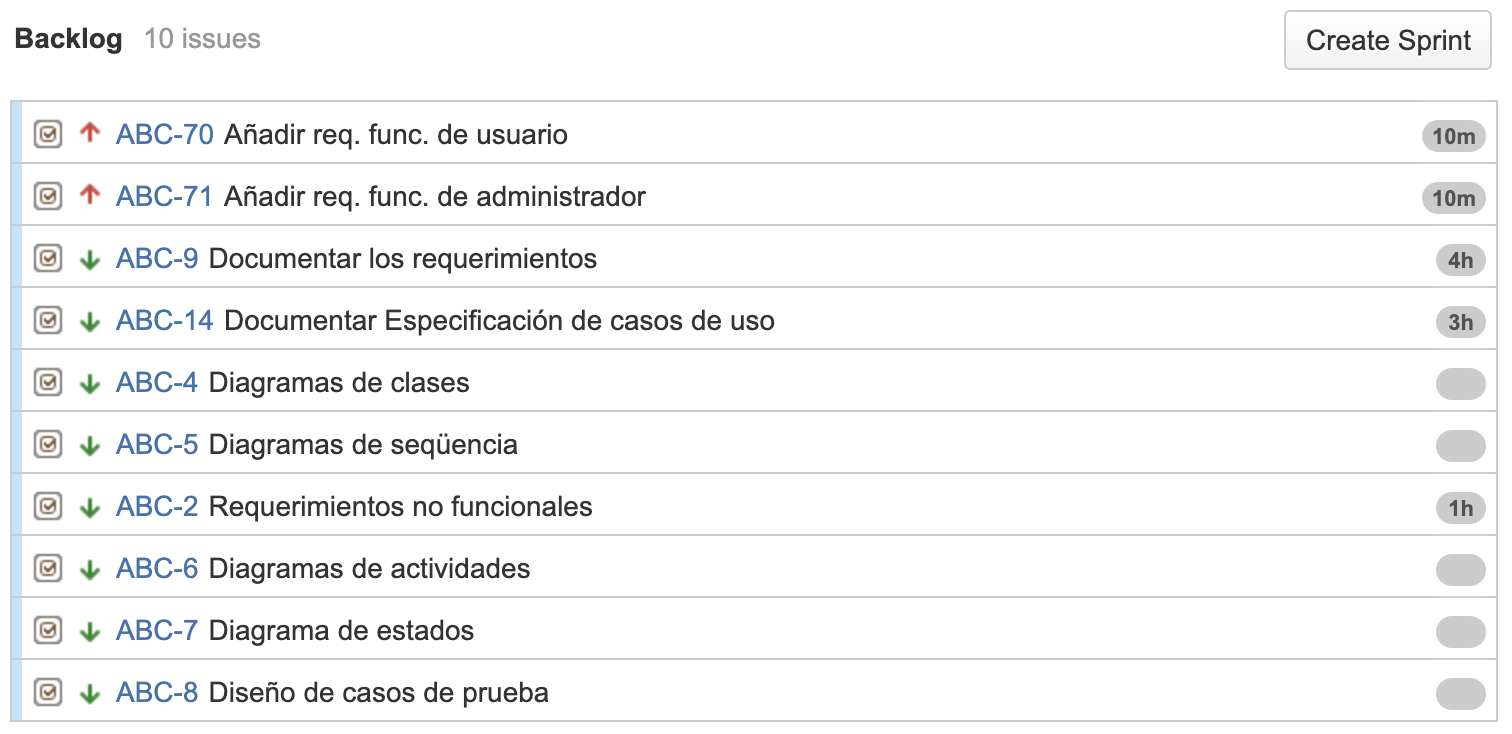
\includegraphics[width=1\textwidth]{./imatges/ProductBacklog2.png}
%}
\subsection{Tasques}
\frame{\frametitle{Tasques}
\begin{center}
	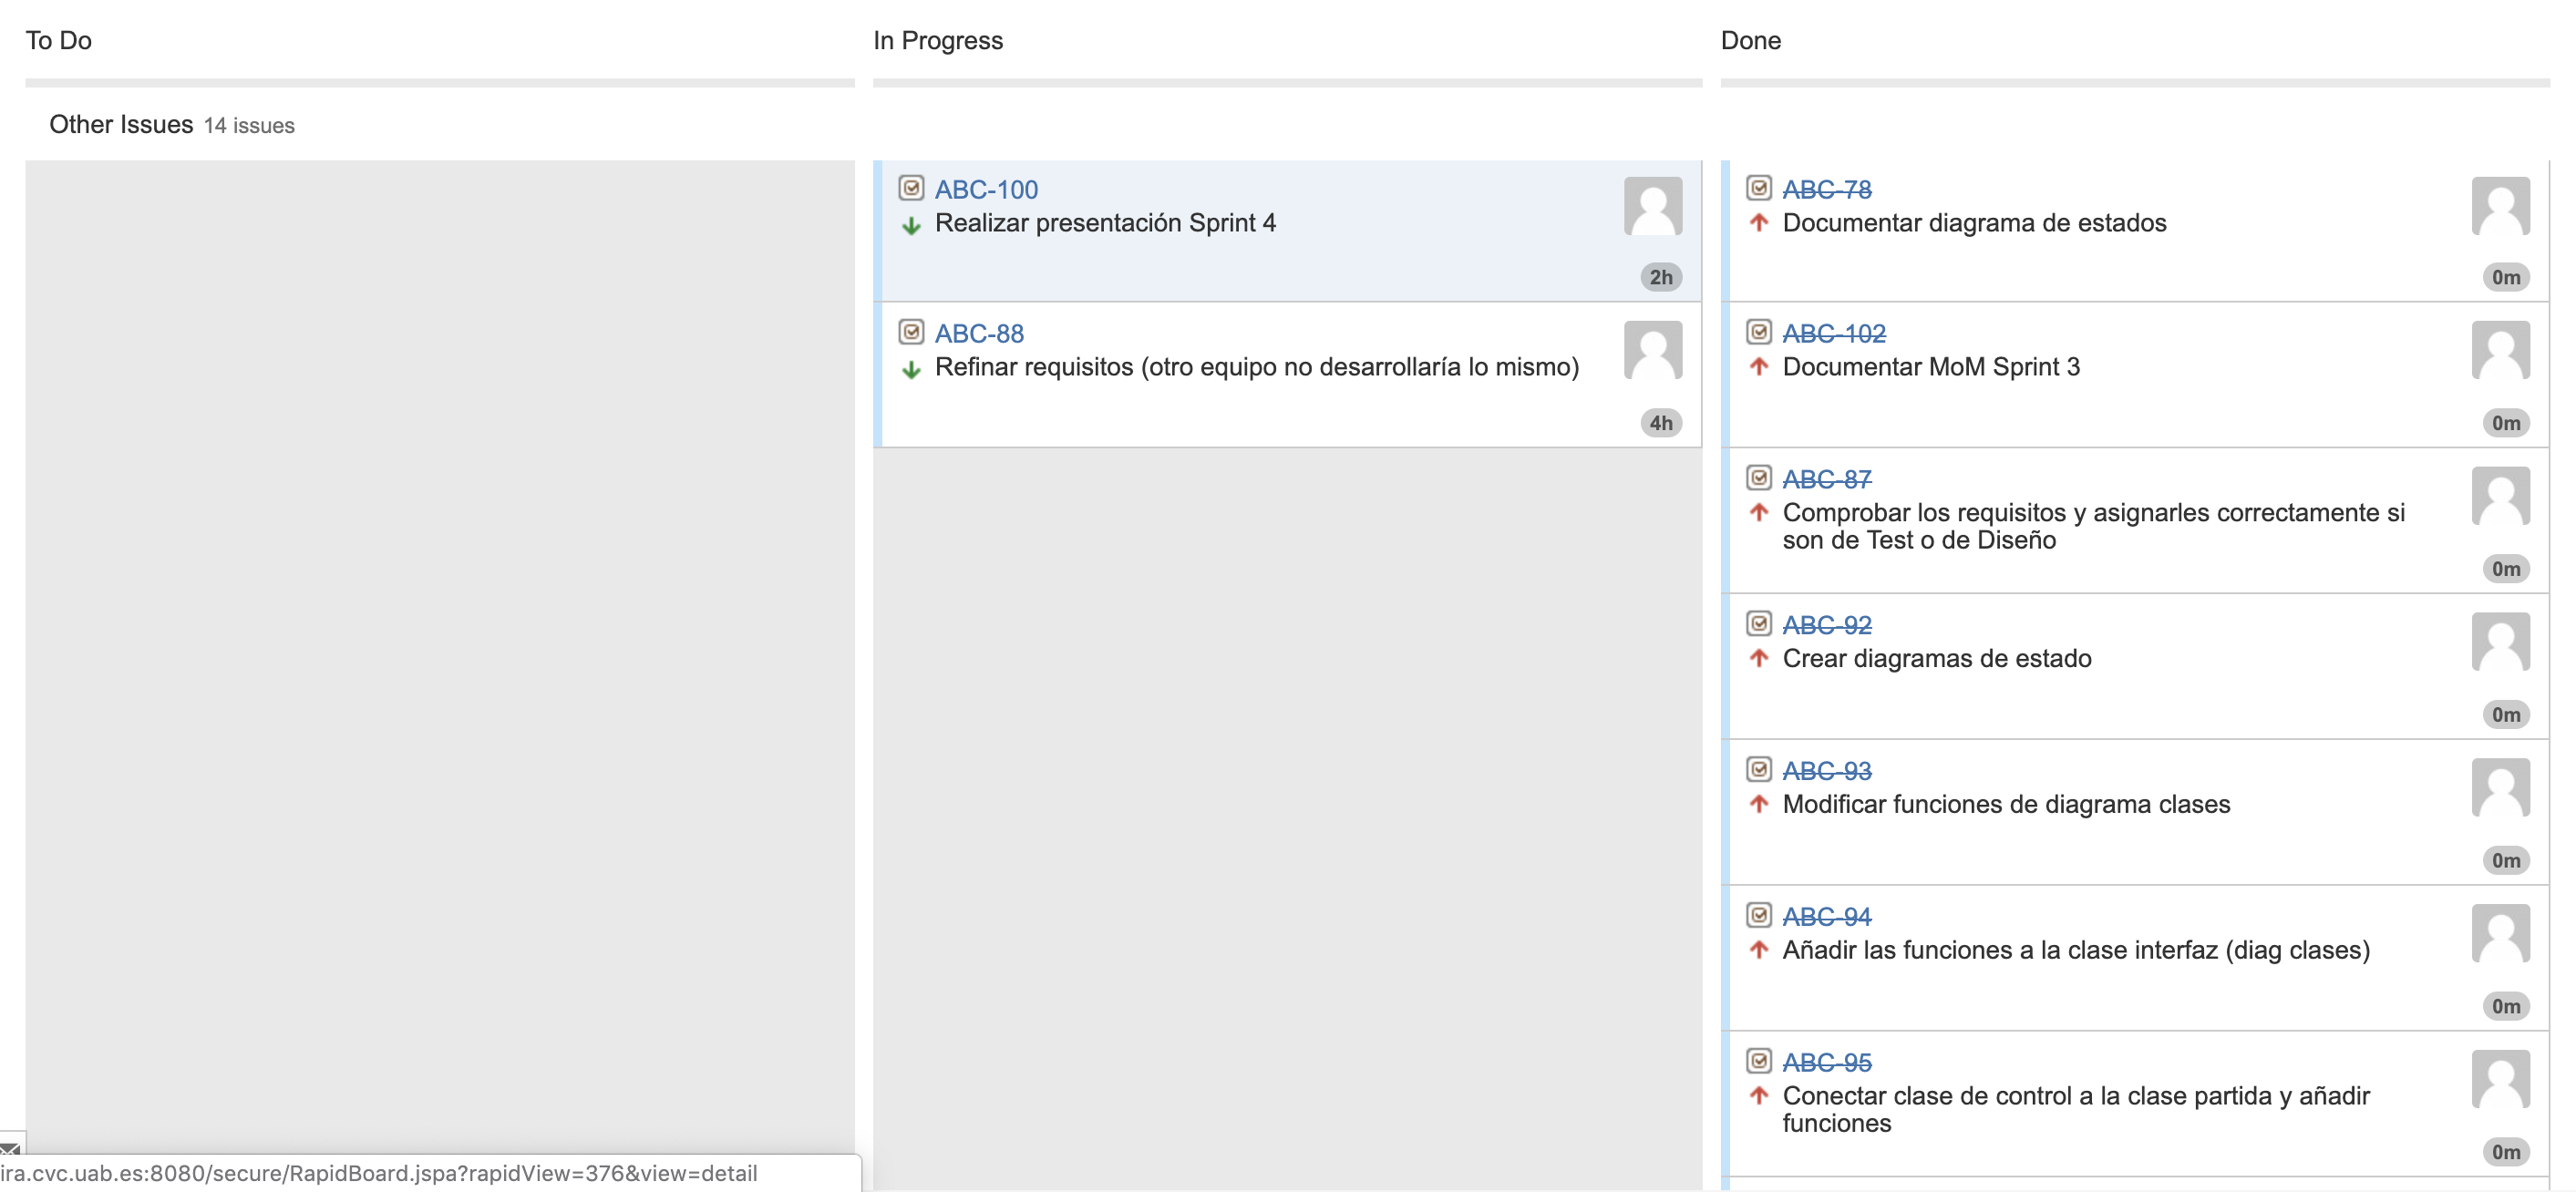
\includegraphics[width=1\textwidth]{./imatges/tareas4.png}
\end{center}
	
}

\subsection{Burndown chart}
\frame{\frametitle{Burndown chart}

  \begin{figure}[ht]
  \centering
  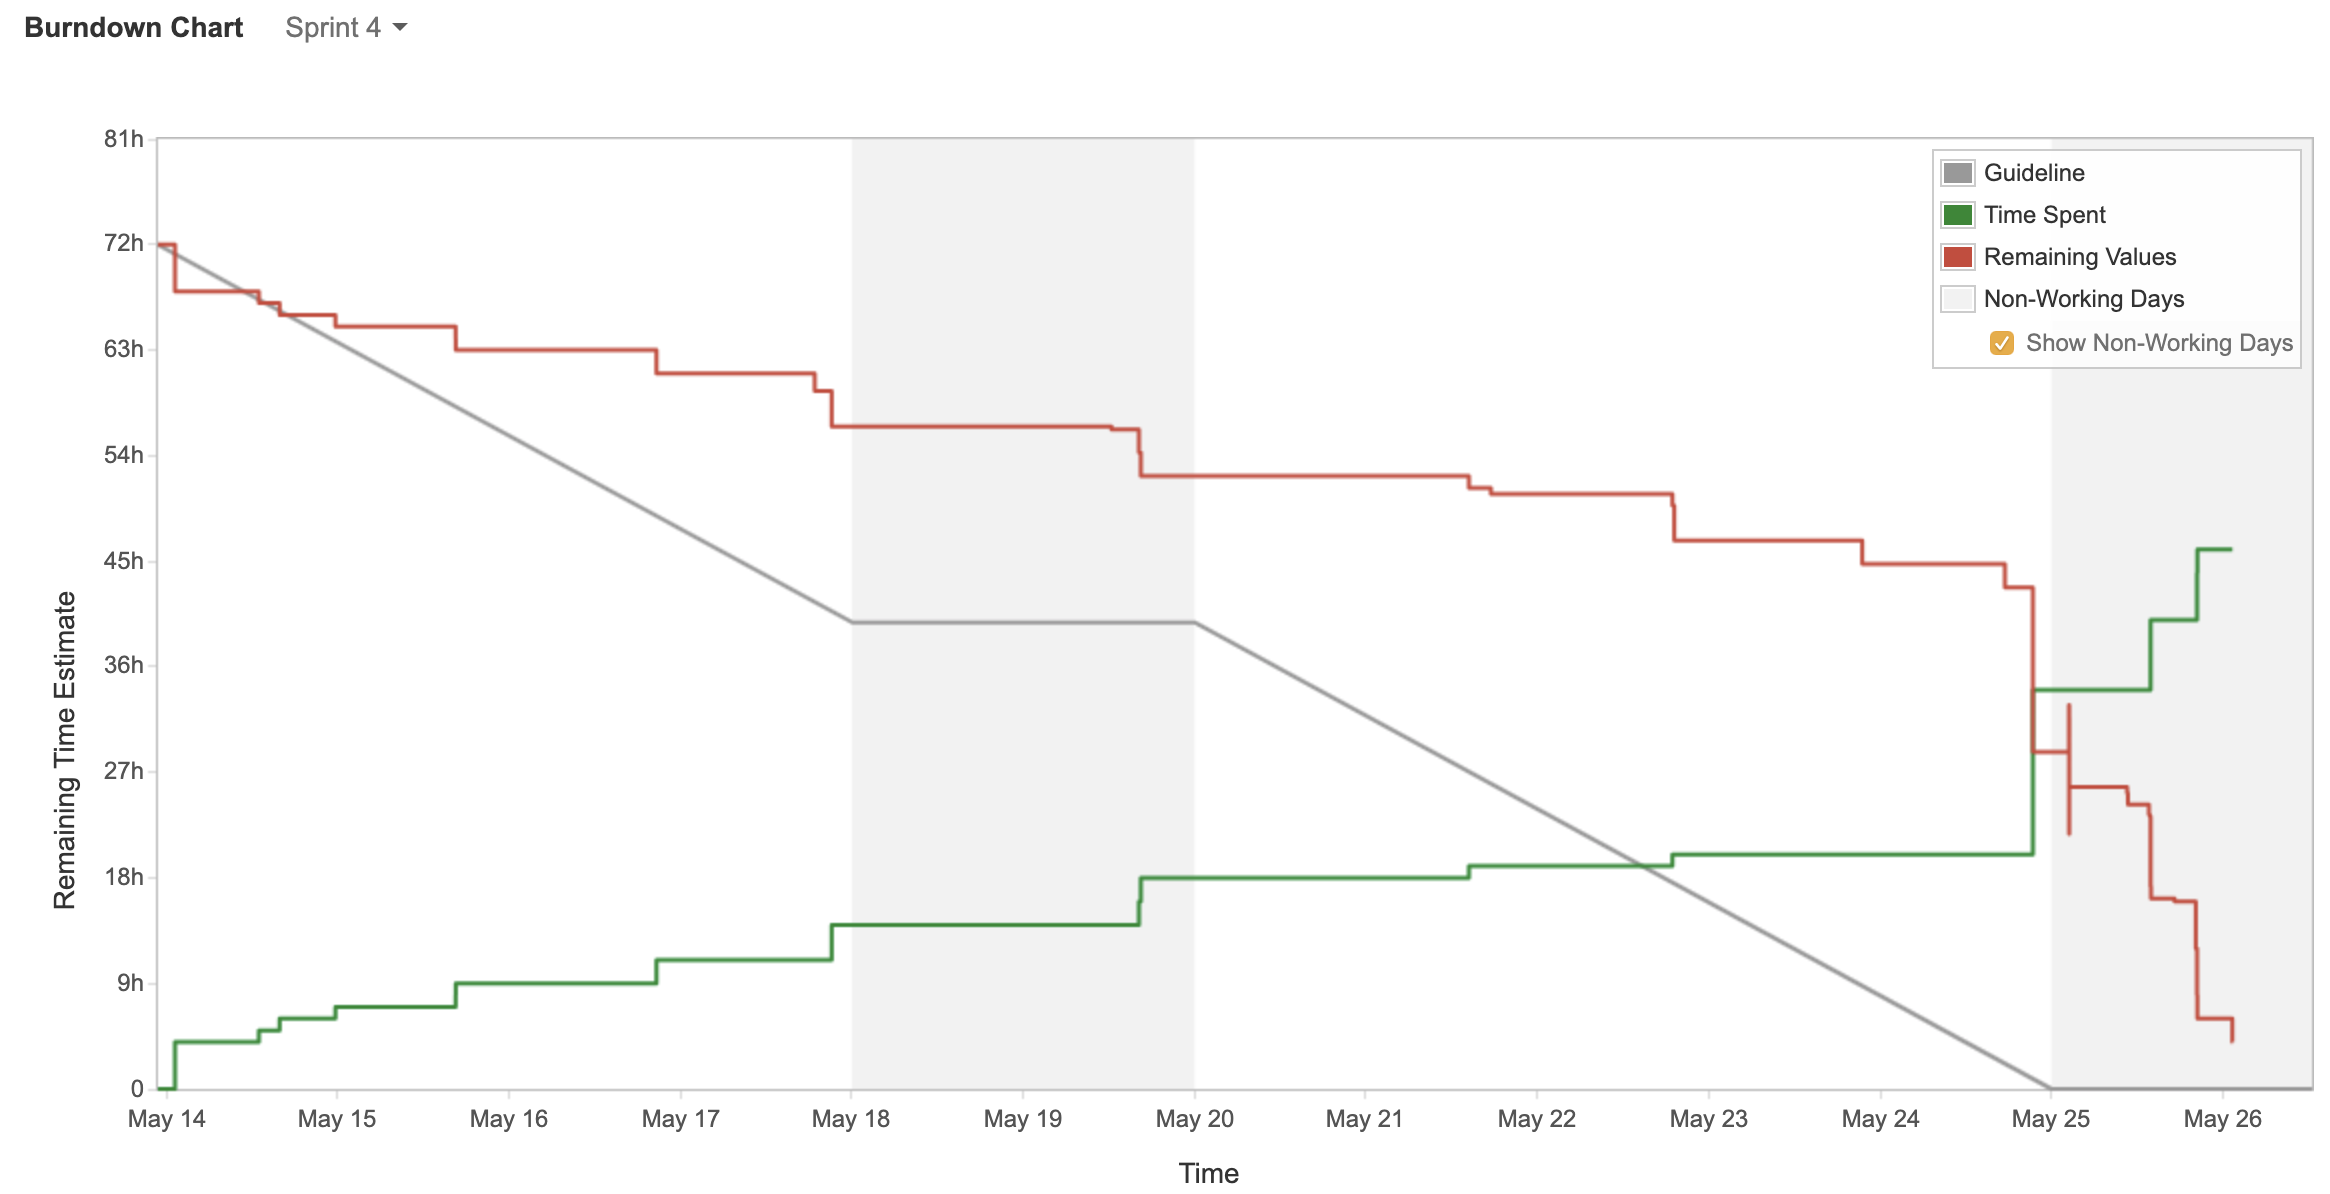
\includegraphics[width=1\textwidth]{./imatges/burndown4.png}
  \label{fig:bdchart}
\end{figure}
}


\section{Bitbucket}
\frame{\frametitle{Bitbucket}
\begin{center}
	\begin{figure}
 \centering
  \subfloat{
    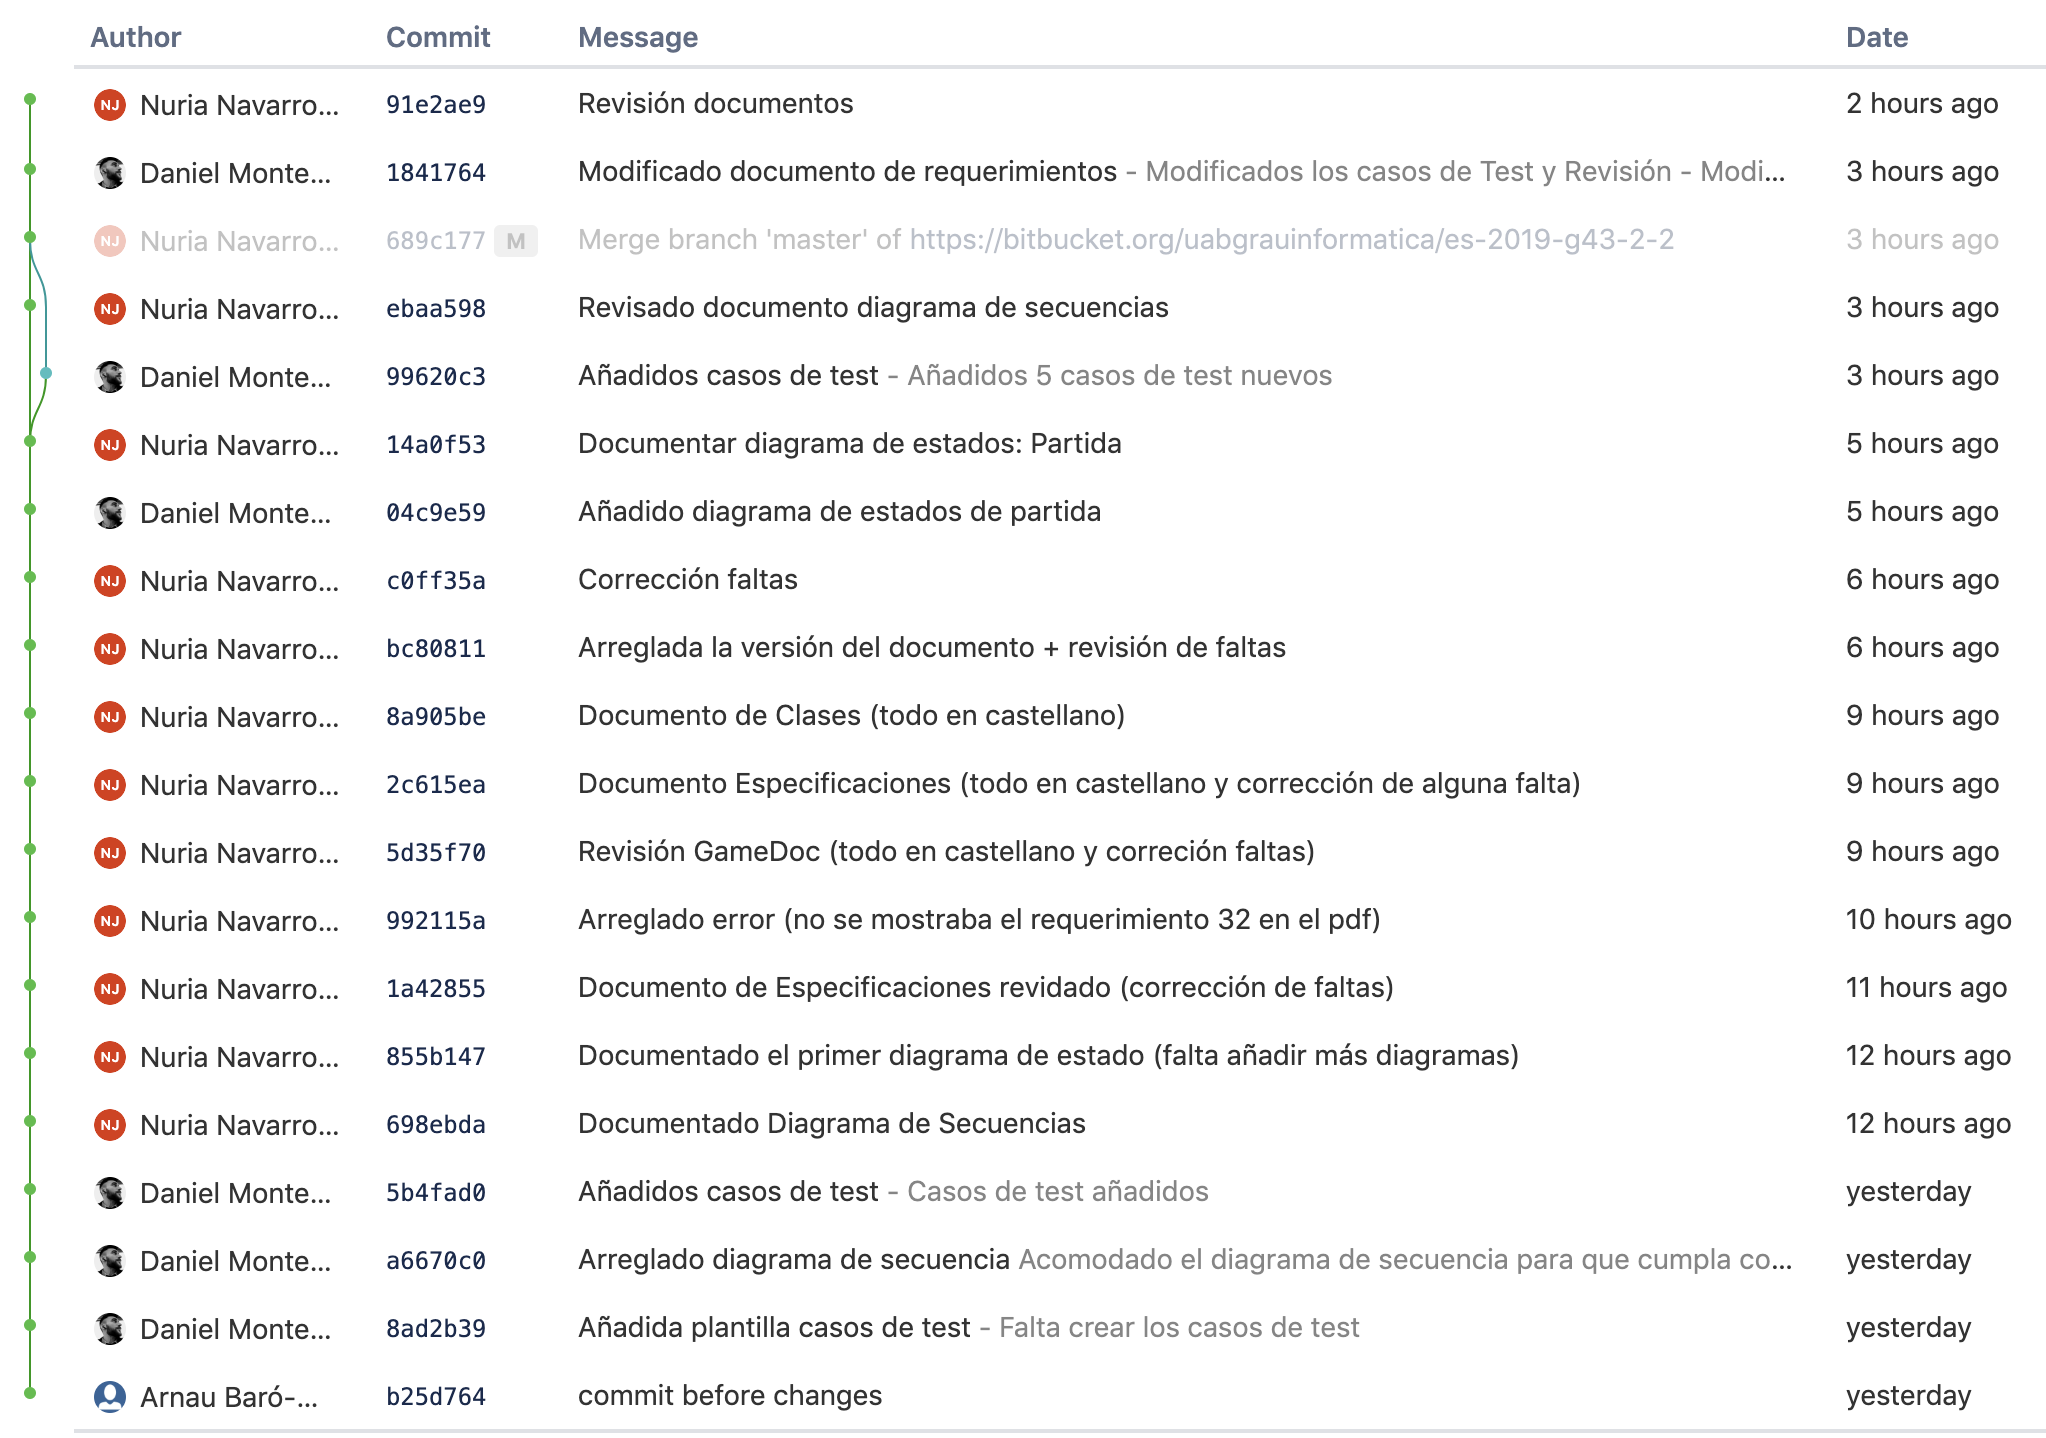
\includegraphics[width=0.5\textwidth]{./imatges/bitbucket41.png}}
  \subfloat{
    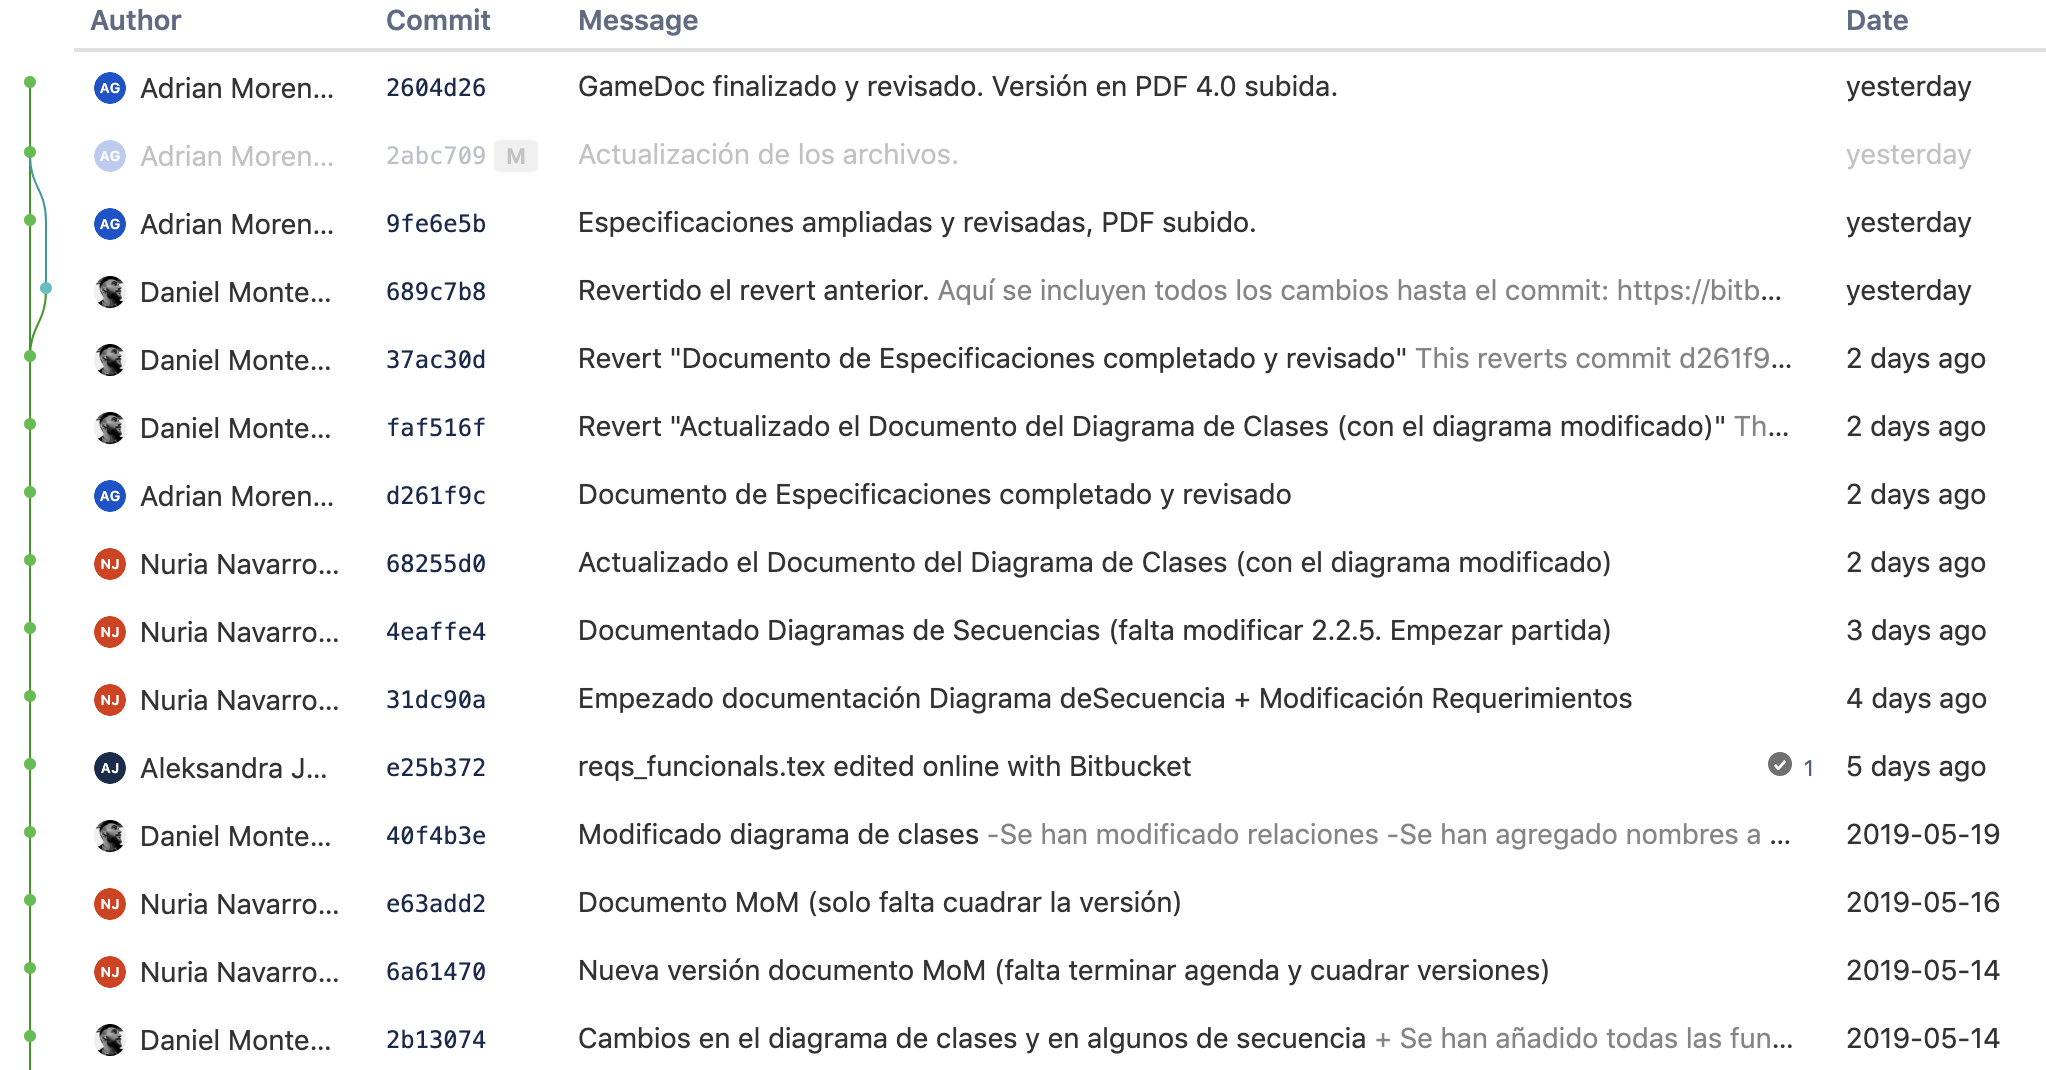
\includegraphics[width=0.45\textwidth]{./imatges/bitbucket42.png}}
\end{figure}
\end{center}
}


\section{Test}
\frame{\frametitle{Test - Eliminar cuentas}
\begin{center}
	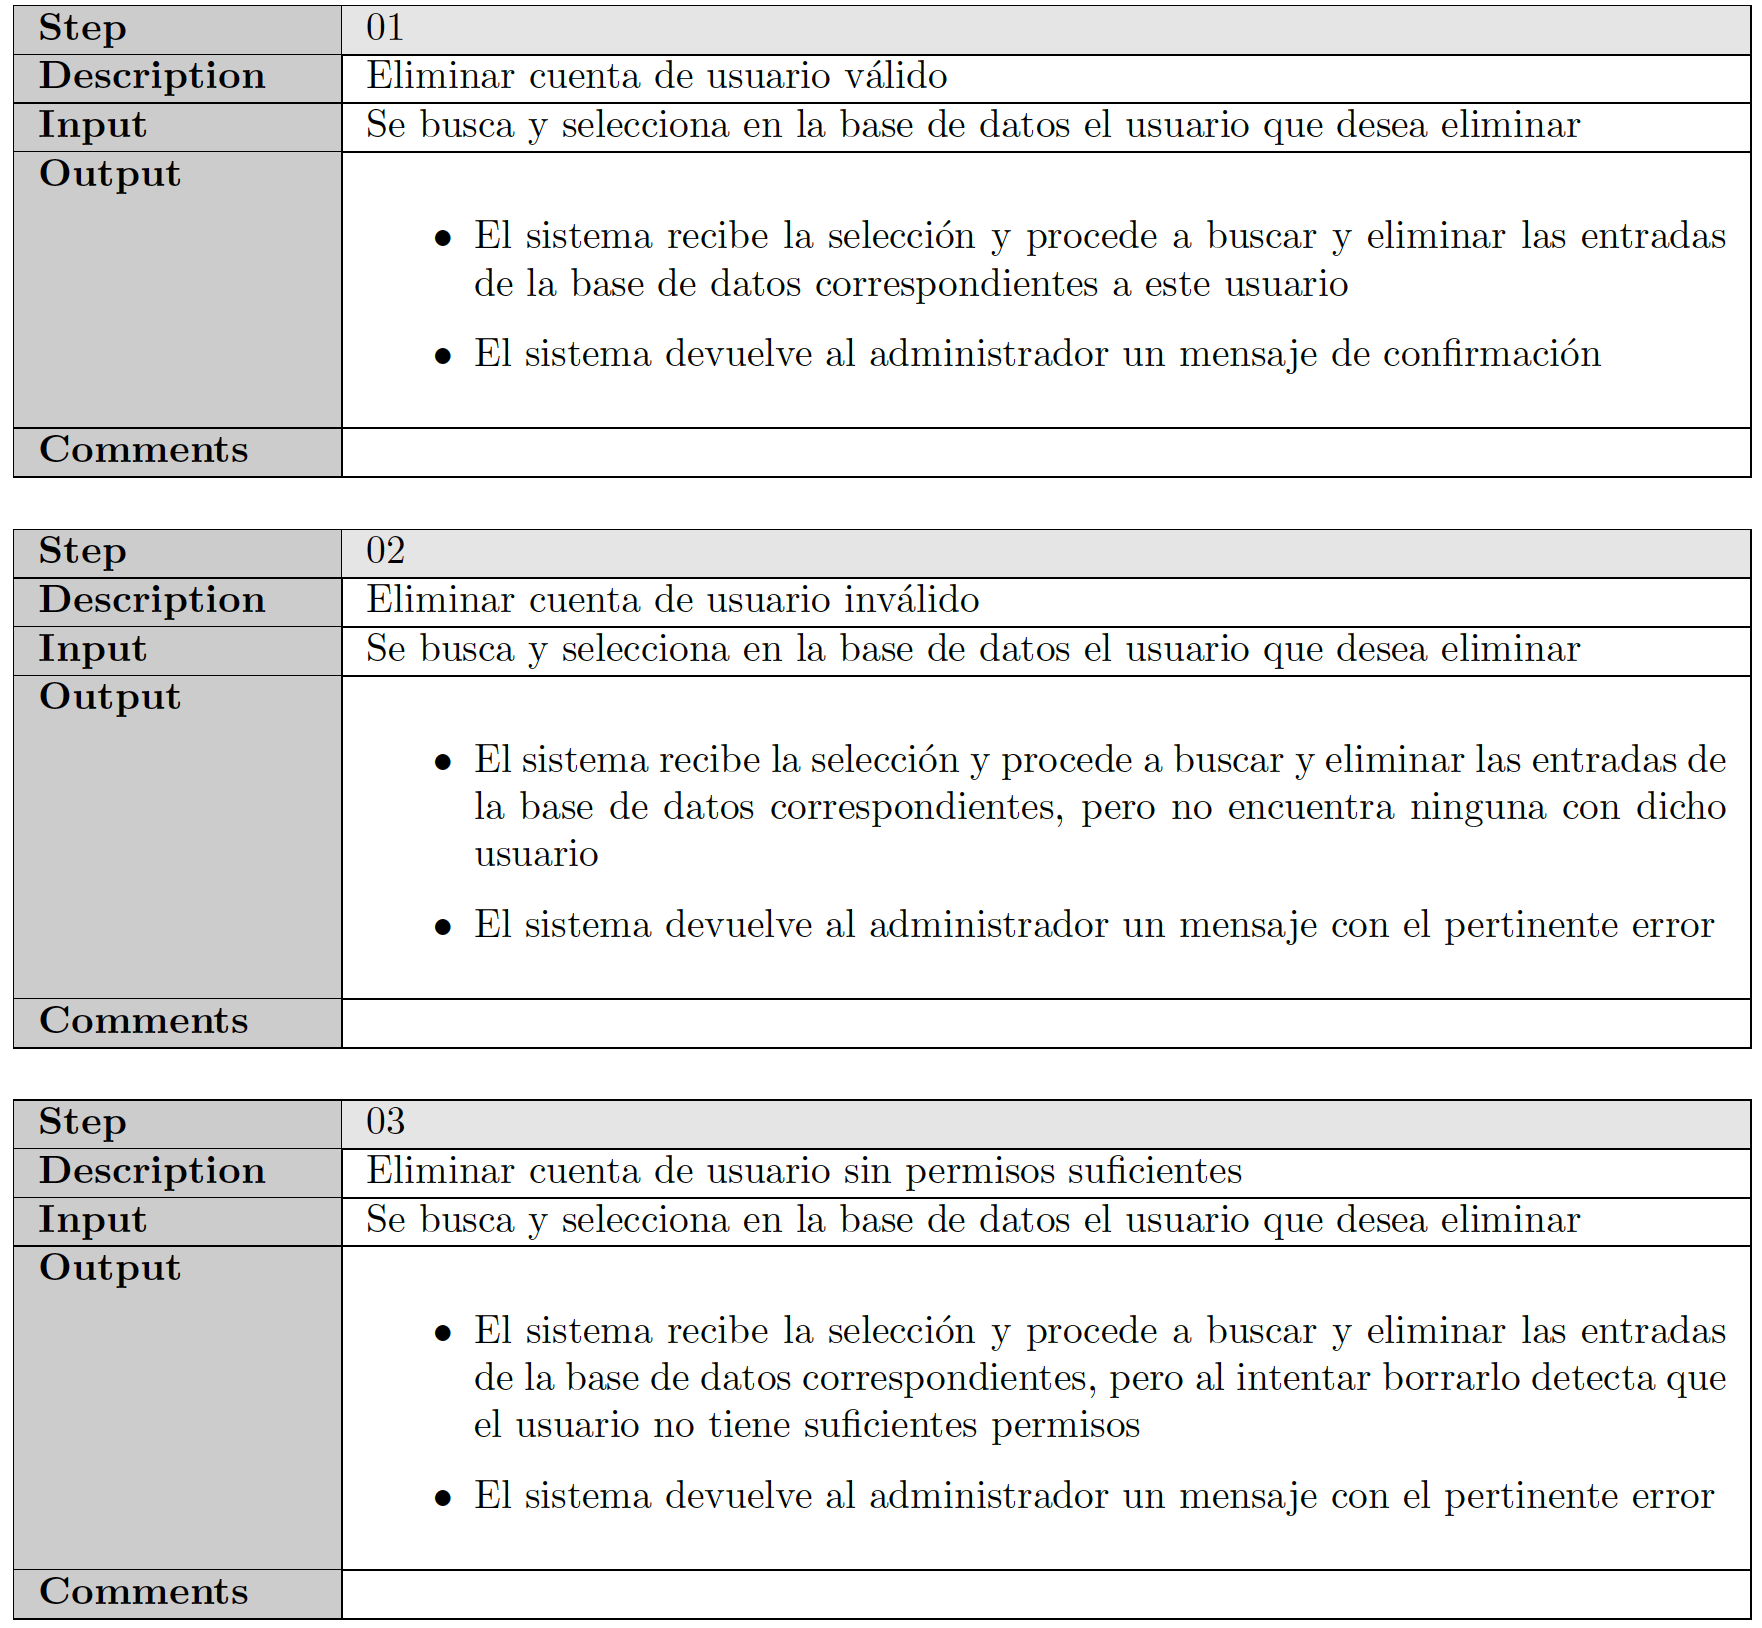
\includegraphics[width=0.6\textwidth]{./imatges/test.png}
\end{center}
}


\section{Sprint Review}
\subsection{Requerimientos}
\frame{\frametitle{Requerimientos}
\begin{center}
	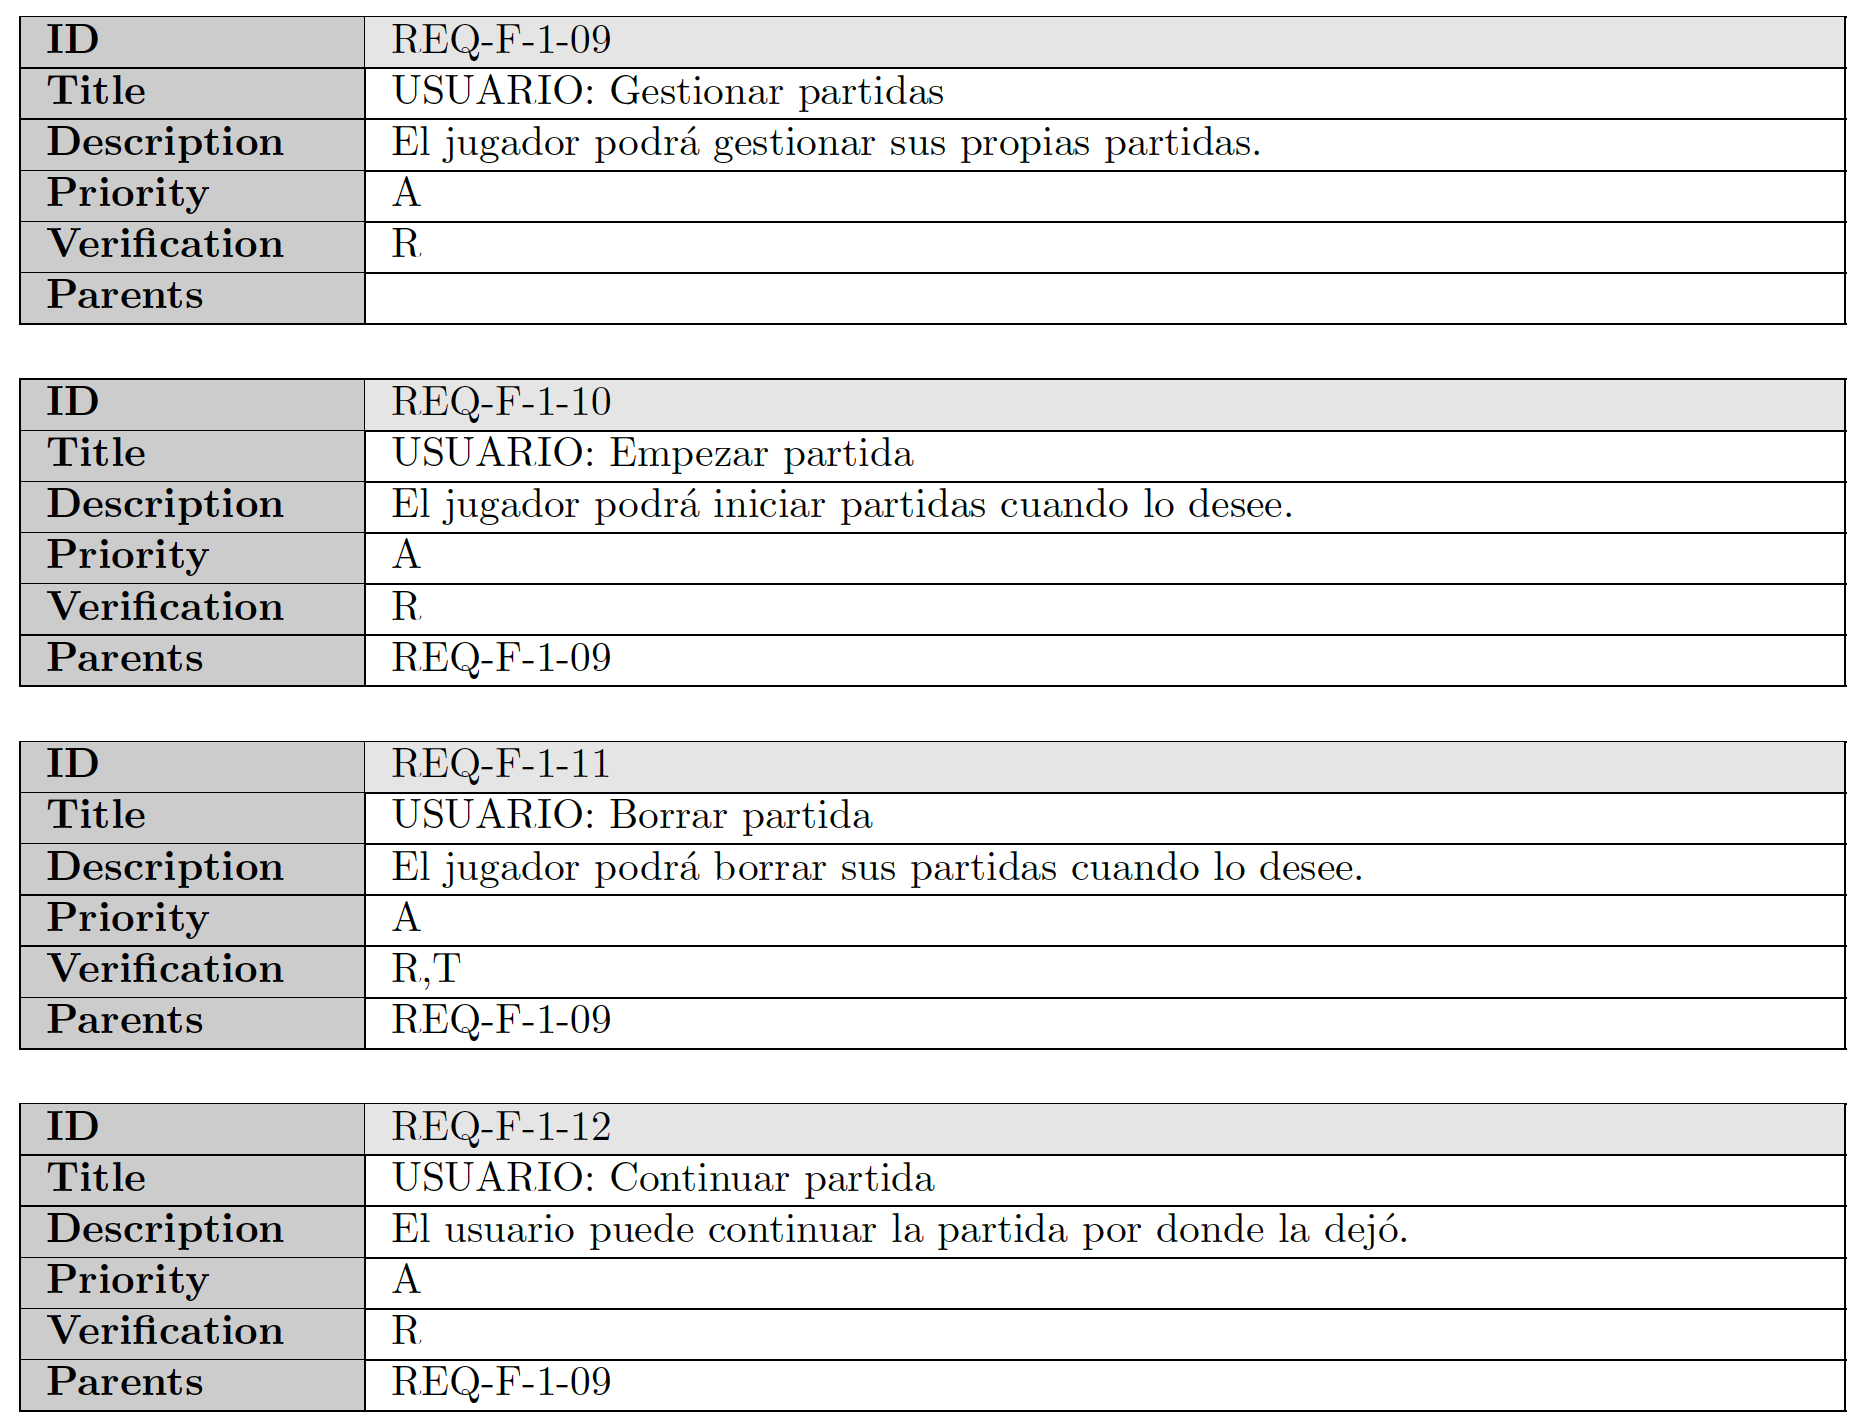
\includegraphics[width=0.6\textwidth]{./imatges/requeriments4.png}
\end{center}
}

\subsection{Diagrama de Casos de Uso}
\frame{\frametitle{Diagrama de Casos de Uso - Administrador}
\begin{center}
	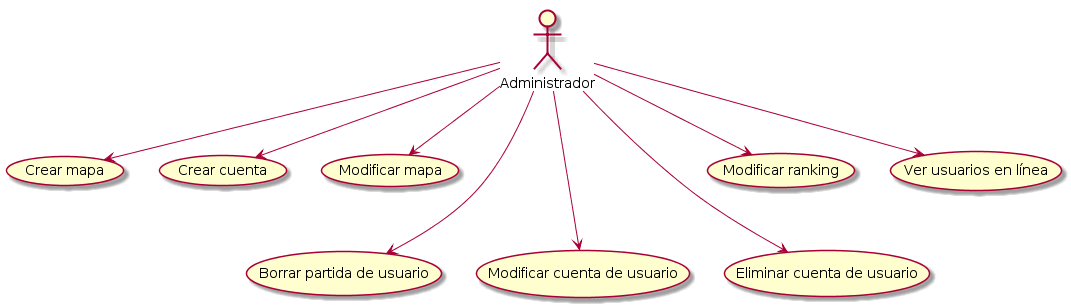
\includegraphics[width=1\textwidth]{./imatges/cu_Administrador4.png}
\end{center}
}

\frame{\frametitle{Diagrama de Casos de Uso - Jugador}
\begin{center}
	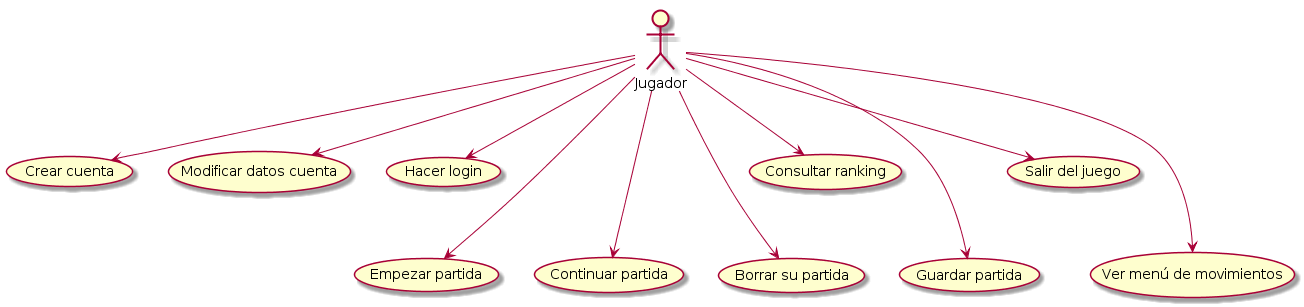
\includegraphics[width=1\textwidth]{./imatges/cu_Jugador4.png}
\end{center}
}

\subsection{Diagrama de Clases}
\frame{\frametitle{Diagrama de Clases}
\begin{center}
	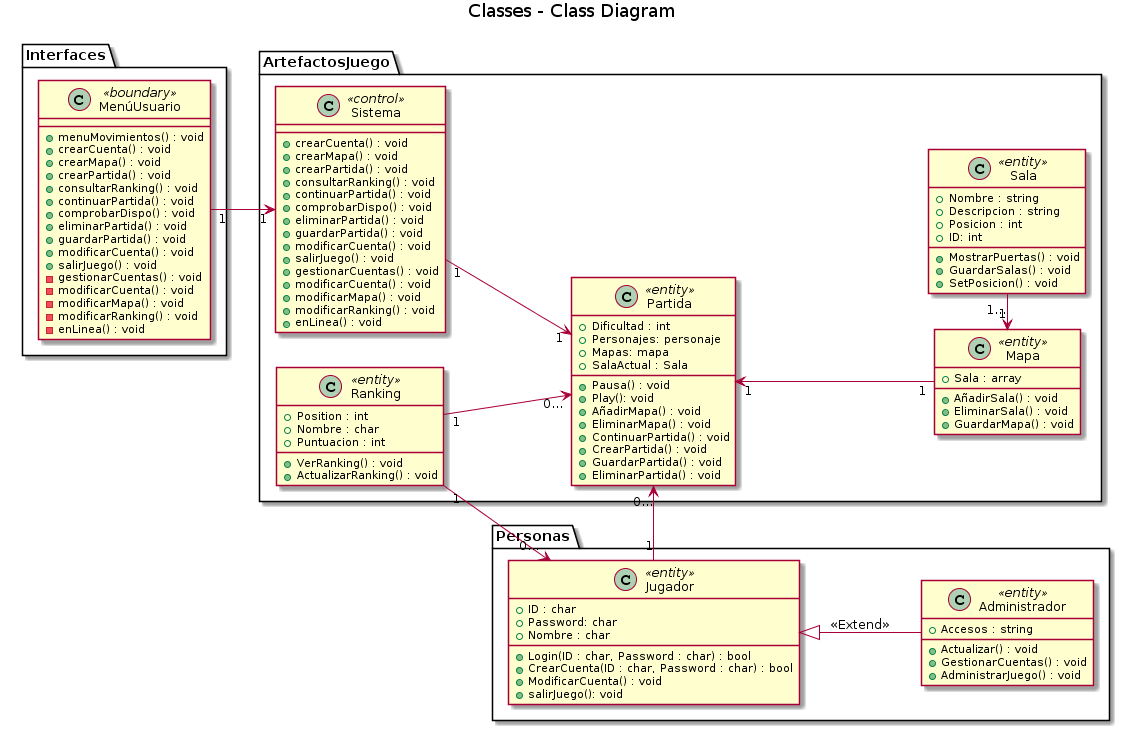
\includegraphics[width=0.8\textwidth]{./imatges/Diagrama_Clases_v4.png}
\end{center}
}

\subsection{Diagrama de Secuencia}
\frame{\frametitle{Diagrama de Secuencia - Administrador}
\begin{center}
	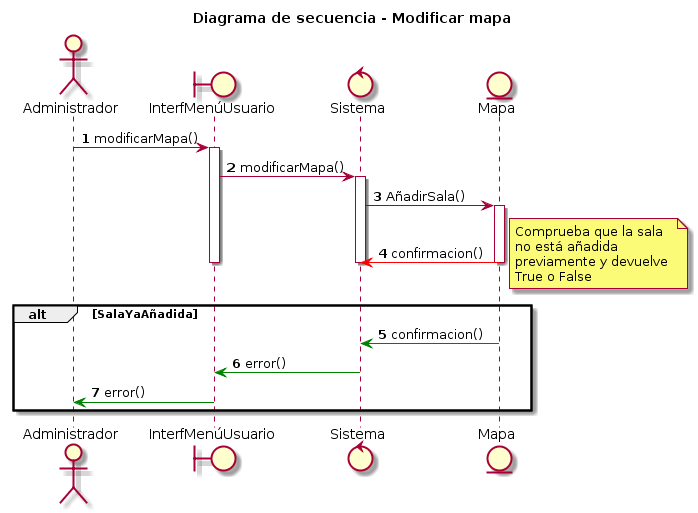
\includegraphics[width=0.7\textwidth]{./imatges/Modificar_mapa.png}
\end{center}
}

\frame{\frametitle{Diagrama de Secuencia - Jugador}
\begin{center}
	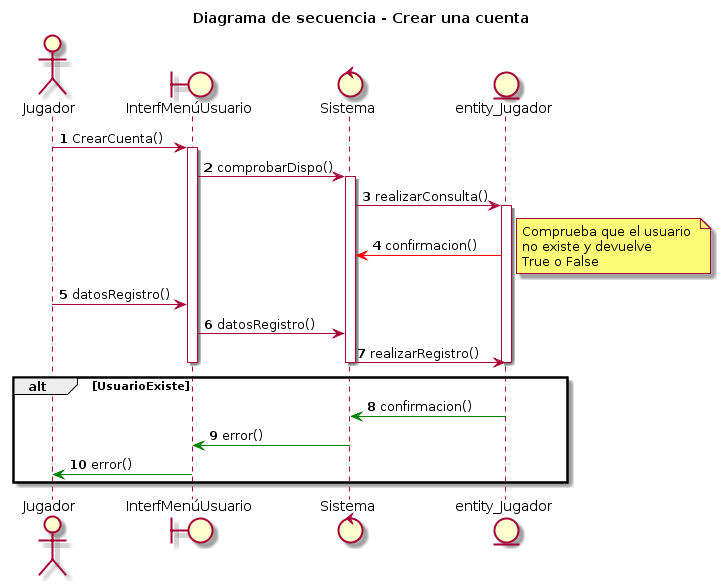
\includegraphics[width=0.6\textwidth]{./imatges/Crear_una_cuenta.png}
\end{center}
}

\subsection{Diagrama de Estado}
\frame{\frametitle{Diagrama de Estado - Estados del juego}
\begin{center}
	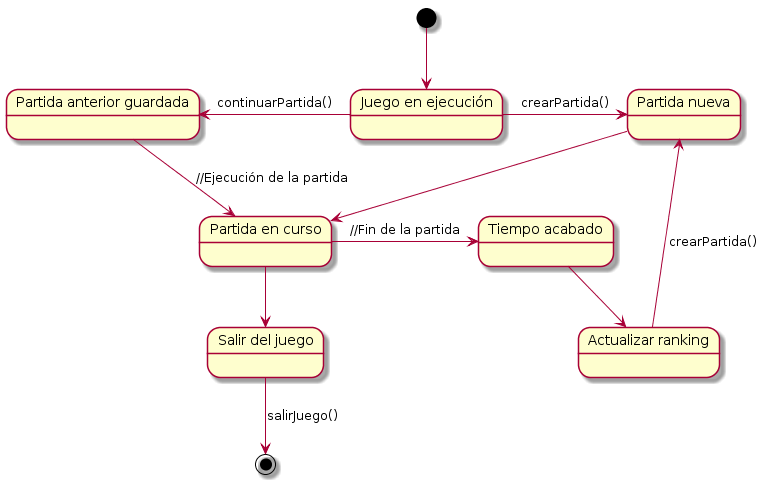
\includegraphics[width=0.9\textwidth]{./imatges/de_Estados_juego.png}
\end{center}
}

\frame{\frametitle{Diagrama de Estado - Partida}
\begin{center}
	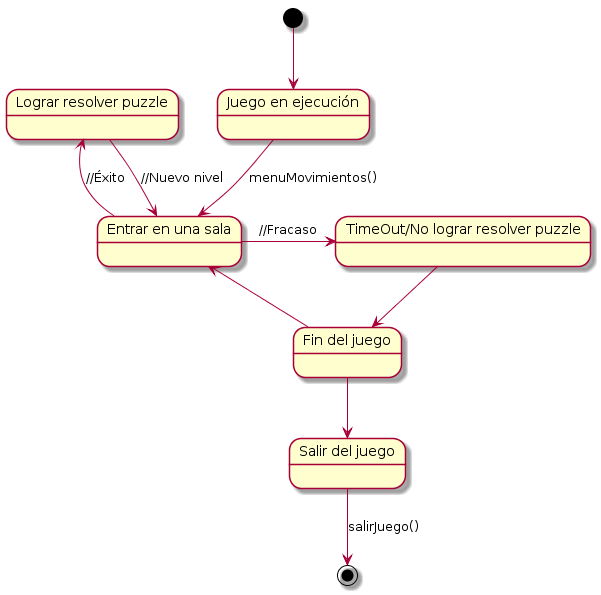
\includegraphics[width=0.55\textwidth]{./imatges/de_Partida.png}
\end{center}
}

\subsection{Evolución}
\frame{\frametitle{Evolución}
\begin{center}
	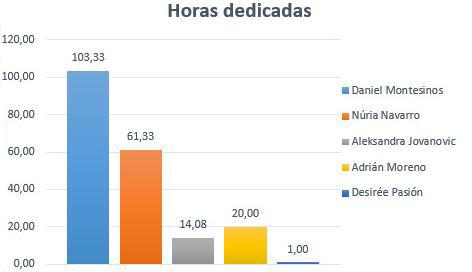
\includegraphics[width=0.7\textwidth]{./imatges/evolucion.png}
\end{center}
}

\section{Perdidos en la ignorancia}
\frame{\frametitle{Perdidos en la ignorancia}
\begin{center}
	
\includegraphics[width=0.6\textwidth]{./imatges/logo.png}
\end{center}
}

\section{Conclusiones}
\frame{\frametitle{Conclusiones}
\begin{enumerate}
	\item Hemos trabajado de manera constante.
	\item Hemos modificado errores de sprints anteriores.
\end{enumerate}}





\end{document}
